\section{Experiment: Direct Plasticity}

\begin{frame}{Direct Plasticity: Biological Intuition}
  \begin{figure} \label{fig:elephant_developmental_perturbation}
  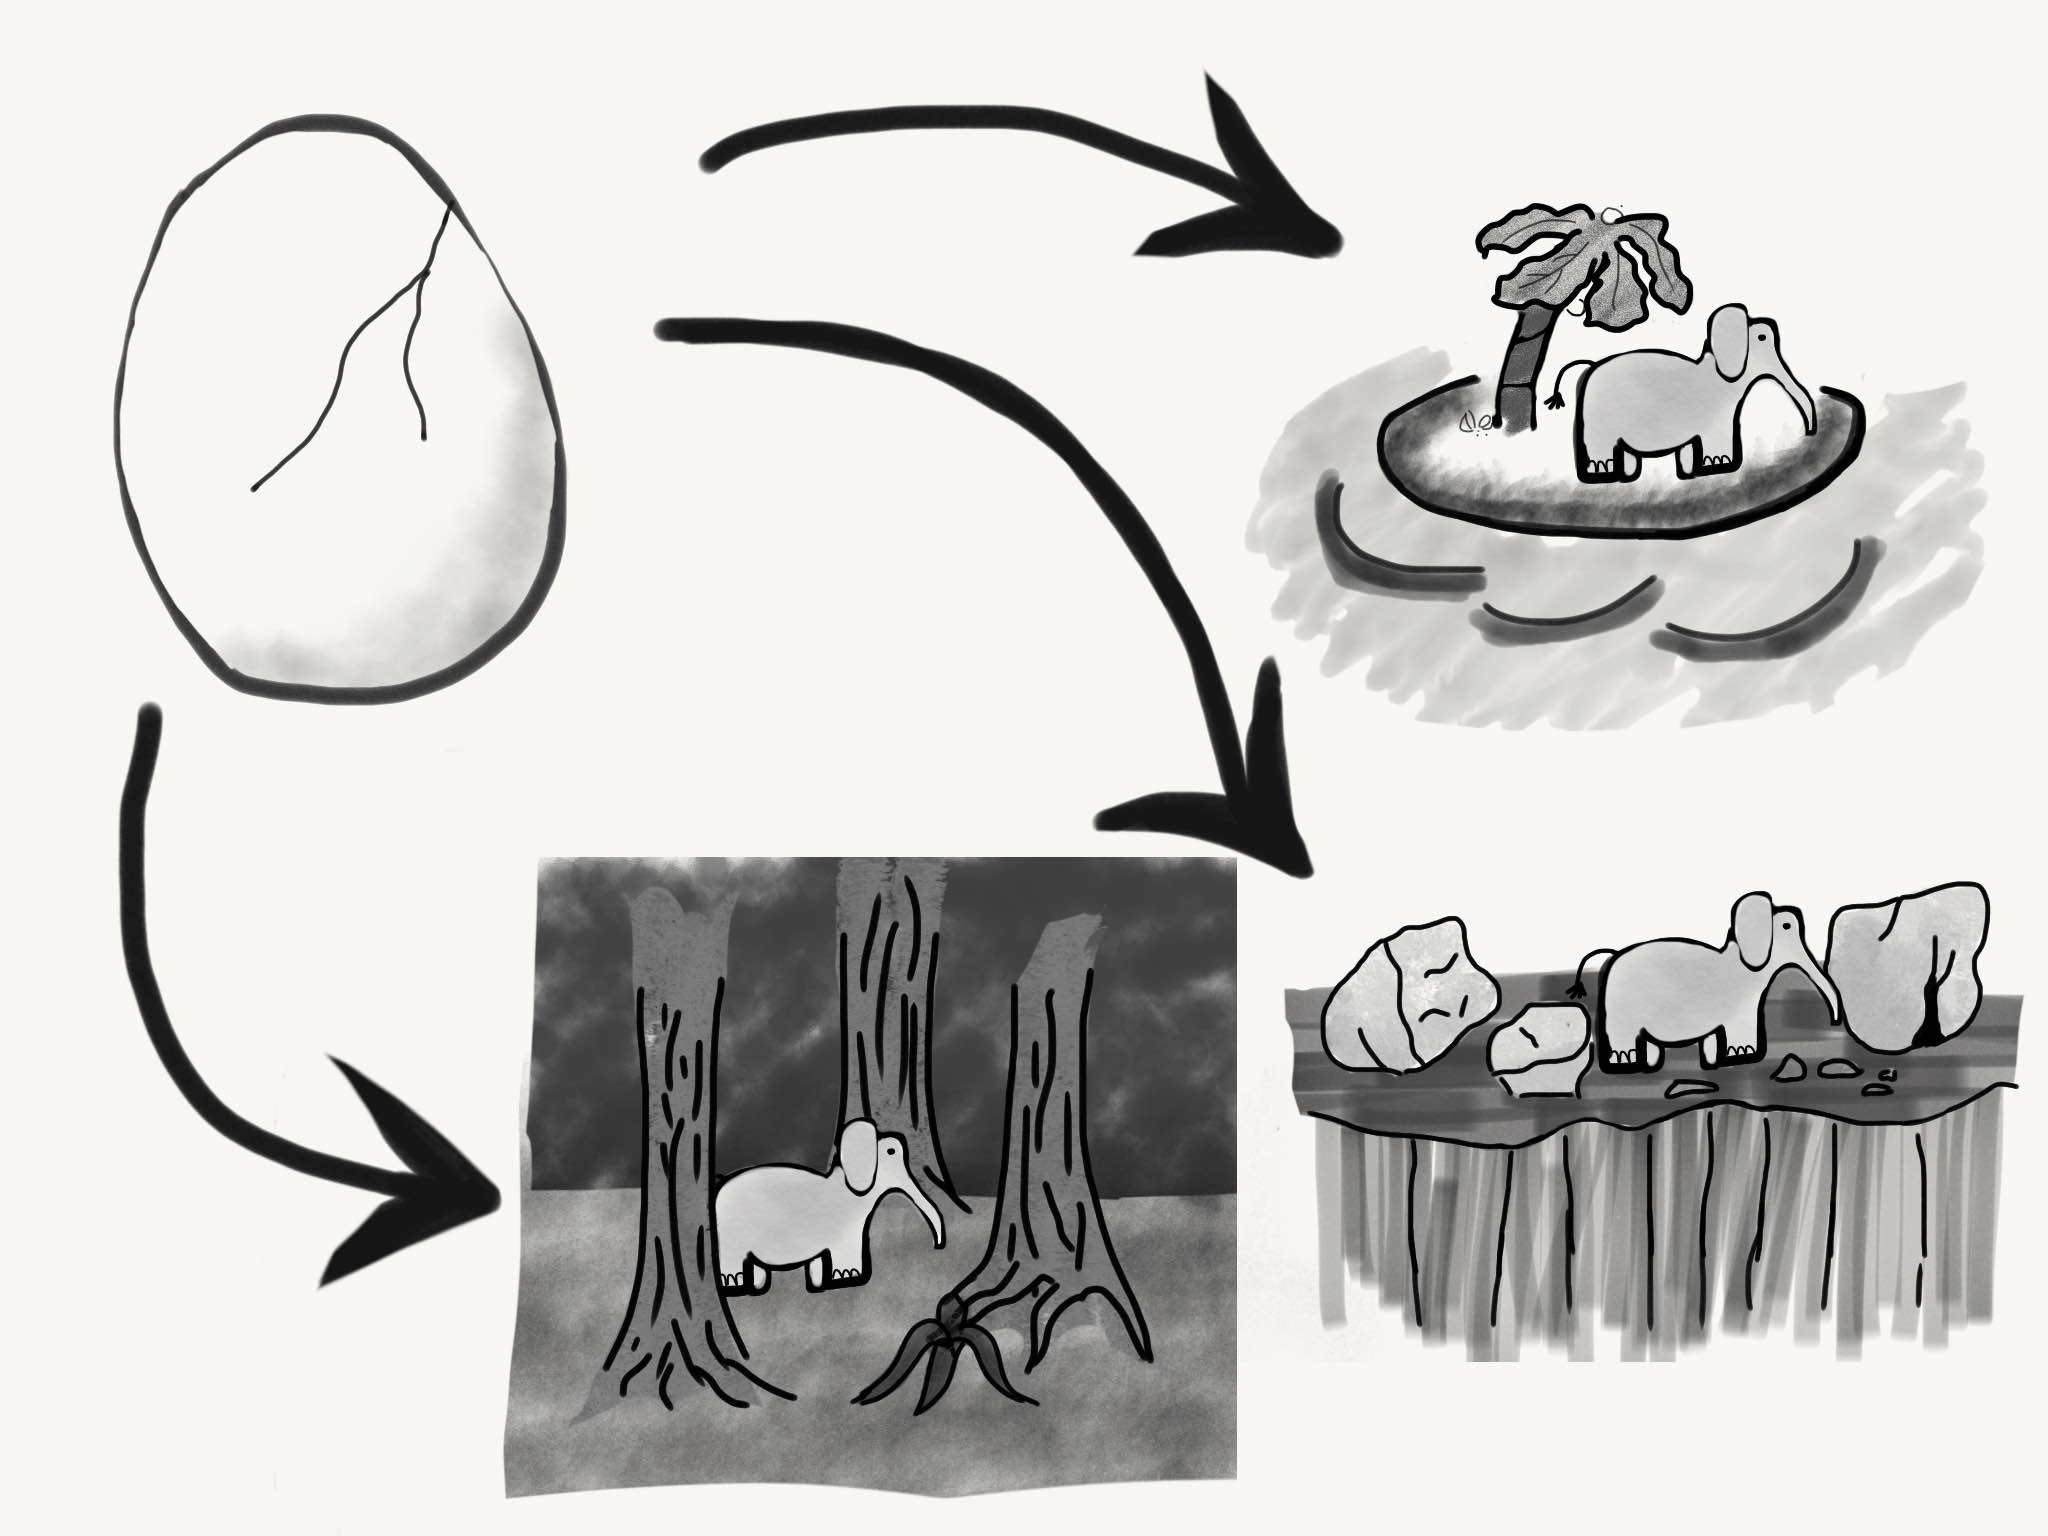
\includegraphics[width=0.8\textwidth]{img/elephant_developmental_perturbation.jpg}
  \captionsetup{singlelinecheck=off,justification=raggedright}

  \caption{A cartoon illustration of resistance to environmental perturbation.}
\end{figure}
\end{frame}

\begin{frame}{Direct Plasticity: Initial State Perturbation}
\begin{figure}
  \centering
  \begin{subfigure}[b]{\textwidth}
    \centering
    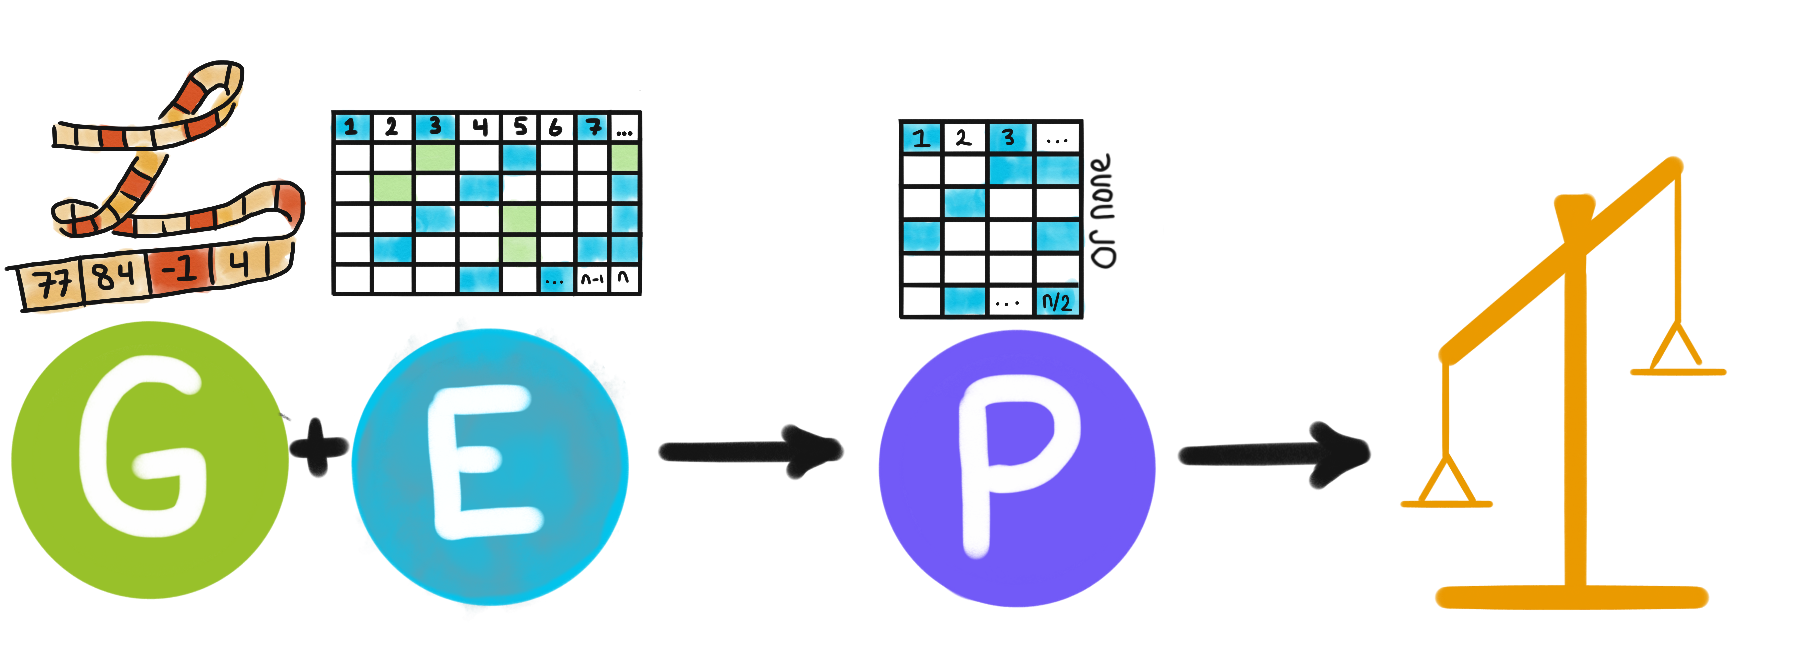
\includegraphics[width=0.6\textwidth]{img/directscheme}
    \caption{experimental scheme}
    \label{subfig:directscheme}
  \end{subfigure}
  \hfill
  \begin{subfigure}[b]{0.6\textwidth}
    \centering
    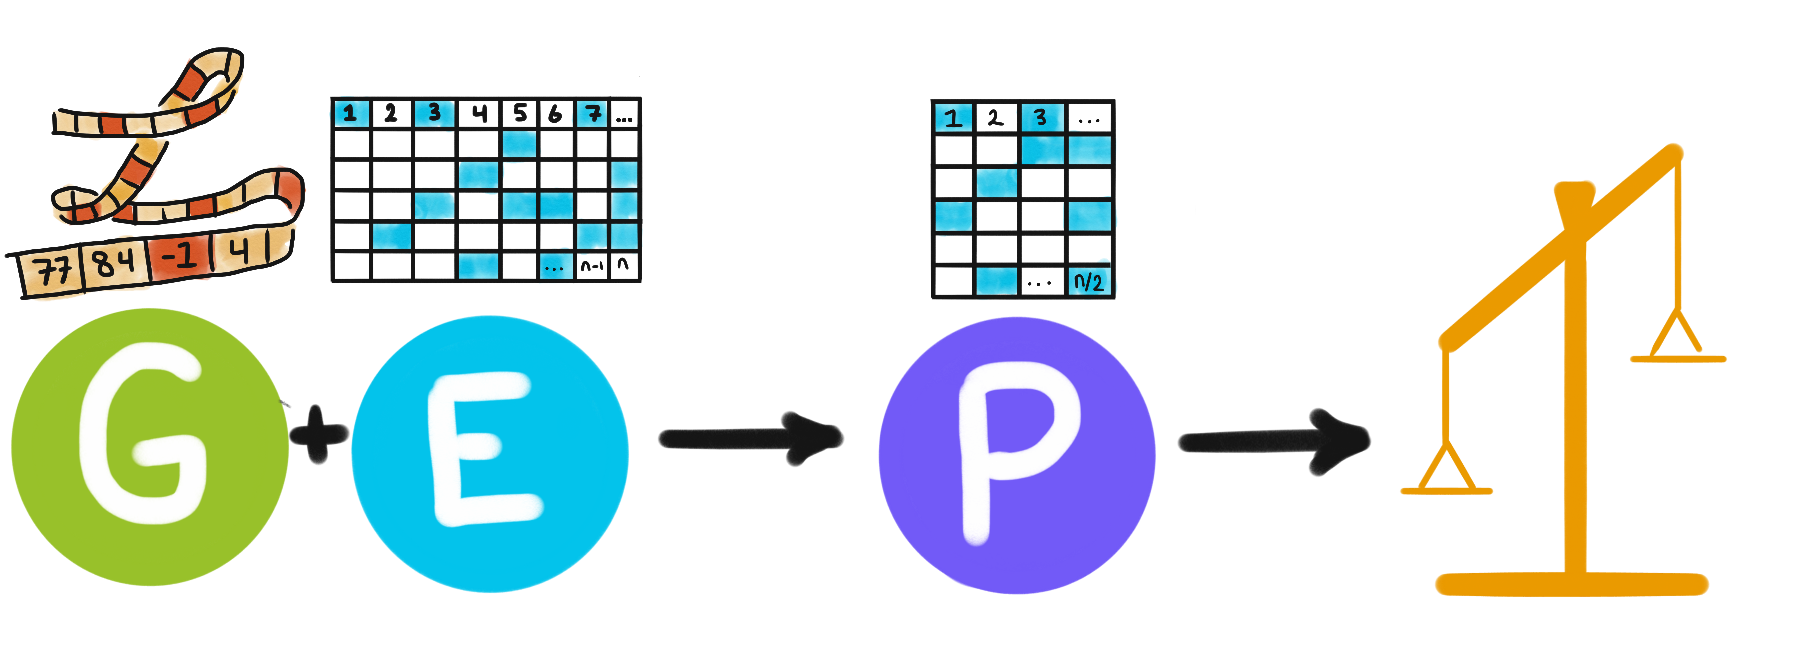
\includegraphics[width=\textwidth]{img/modelscheme}
    \caption{control scheme}
     \label{subfig:controlscheme}
  \end{subfigure}
  \captionsetup{singlelinecheck=off,justification=raggedright}
  \caption{A comparison of the control and experimental schemes employed to investigate the relationship between direct plasticity and evolvability.}
  \label{fig:direct_plasticity_scheme}
\end{figure}
\end{frame}

\begin{frame}{Mutational Outcome Frequencies}
\begin{figure}
    \centering
    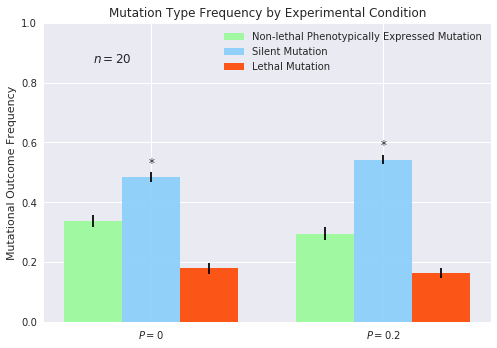
\includegraphics[width=0.8\textwidth]{img/mutation_type_direct}
 	\captionsetup{singlelinecheck=off,justification=raggedright}
  	\caption{Comparison of mutational outcome frequencies for champions evolved with and without initial state perturbation.}
    \label{fig:mutation_type_direct}
\end{figure}
\end{frame}

% \begin{frame}{Direct Plasticity Results: Summary}
% \begin{itemize}
%   \item direct plasticity increases robustness to mutation
%   \item as in \cite{Reisinger2005TowardsEvolvability}, repeated evaluations ($n=10$) were required to observe impact of direct plasticity
% \end{itemize}
% \end{frame}